% Gerado automaticamente. No preambulo do documento use:
% \usepackage{pgfplots}
% \pgfplotsset{compat=1.18}
\definecolor{plotblue}{HTML}{2563EB}
\definecolor{plotorange}{HTML}{D97706}
\definecolor{plotgreen}{HTML}{059669}
\definecolor{plotpurple}{HTML}{7C3AED}
\definecolor{plotgray}{HTML}{374151}
\definecolor{plotred}{HTML}{DC2626}
\definecolor{plotteal}{HTML}{0F766E}
\definecolor{plotslate}{HTML}{64748B}

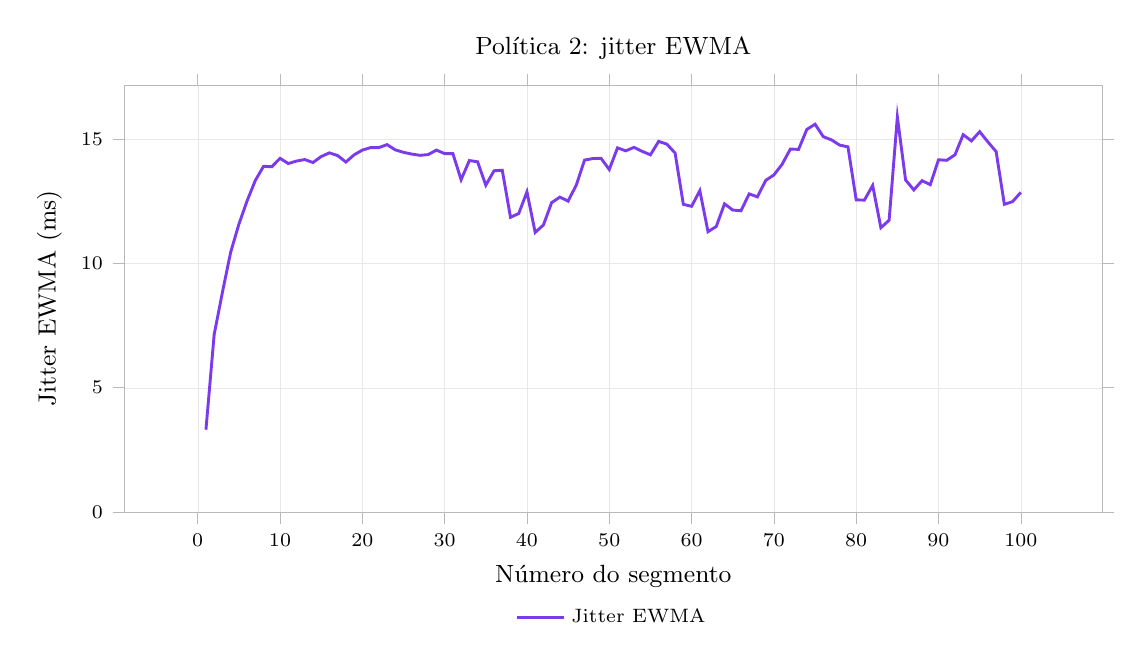
\begin{tikzpicture}
\begin{axis}[
    title={Política 2: jitter EWMA},
    xlabel={Número do segmento},
    ylabel={Jitter EWMA (ms)},
    width=14cm,
    height=7cm,
    grid=major,
    grid style={line width=.12pt, draw=gray!18},
    axis line style={draw=gray!55},
    tick style={draw=gray!55},
    tick align=outside,
    title style={font=\small},
    label style={font=\small},
    tick label style={font=\scriptsize},
    legend cell align={left},
    legend style={at={(0.5,-0.20)}, anchor=north, legend columns=2, draw=none, font=\scriptsize},
    ymin=0,
    ymax=17.1504
]
\addplot+[plotpurple, line width=1.05pt, mark=none] coordinates {
(1,3.31)
(2,7.14)
(3,8.83)
(4,10.44)
(5,11.57)
(6,12.51)
(7,13.33)
(8,13.9)
(9,13.88)
(10,14.22)
(11,14.01)
(12,14.11)
(13,14.17)
(14,14.05)
(15,14.29)
(16,14.44)
(17,14.33)
(18,14.07)
(19,14.36)
(20,14.55)
(21,14.65)
(22,14.65)
(23,14.77)
(24,14.56)
(25,14.46)
(26,14.39)
(27,14.34)
(28,14.37)
(29,14.55)
(30,14.41)
(31,14.41)
(32,13.36)
(33,14.13)
(34,14.08)
(35,13.14)
(36,13.72)
(37,13.74)
(38,11.85)
(39,12)
(40,12.87)
(41,11.24)
(42,11.54)
(43,12.44)
(44,12.66)
(45,12.5)
(46,13.15)
(47,14.15)
(48,14.21)
(49,14.22)
(50,13.77)
(51,14.64)
(52,14.52)
(53,14.66)
(54,14.5)
(55,14.36)
(56,14.9)
(57,14.79)
(58,14.43)
(59,12.37)
(60,12.29)
(61,12.92)
(62,11.27)
(63,11.48)
(64,12.39)
(65,12.14)
(66,12.11)
(67,12.79)
(68,12.67)
(69,13.33)
(70,13.55)
(71,13.98)
(72,14.59)
(73,14.58)
(74,15.38)
(75,15.59)
(76,15.09)
(77,14.96)
(78,14.75)
(79,14.68)
(80,12.55)
(81,12.54)
(82,13.13)
(83,11.43)
(84,11.73)
(85,15.88)
(86,13.35)
(87,12.95)
(88,13.32)
(89,13.16)
(90,14.16)
(91,14.14)
(92,14.36)
(93,15.17)
(94,14.92)
(95,15.29)
(96,14.88)
(97,14.49)
(98,12.37)
(99,12.48)
(100,12.85)
};
\addlegendentry{Jitter EWMA}
\end{axis}
\end{tikzpicture}
